%%%%%%%%%%%%%%%%%%%%%%%%%%%%%%%%%%%%%%%%%
% Lachaise Assignment
% LaTeX Template
% Version 1.0 (26/6/2018)
%
% This template originates from:
% http://www.LaTeXTemplates.com
%
% Authors:
% Marion Lachaise & François Févotte
% Vel (vel@LaTeXTemplates.com)
%
% License:
% CC BY-NC-SA 3.0 (http://creativecommons.org/licenses/by-nc-sa/3.0/)
% 
%%%%%%%%%%%%%%%%%%%%%%%%%%%%%%%%%%%%%%%%%

%----------------------------------------------------------------------------------------
%	PACKAGES AND OTHER DOCUMENT CONFIGURATIONS
%----------------------------------------------------------------------------------------

\documentclass{article}

%%%%%%%%%%%%%%%%%%%%%%%%%%%%%%%%%%%%%%%%%
% Lachaise Assignment
% Structure Specification File
% Version 1.0 (26/6/2018)
%
% This template originates from:
% http://www.LaTeXTemplates.com
%
% Authors:
% Marion Lachaise & François Févotte
% Vel (vel@LaTeXTemplates.com)
%
% License:
% CC BY-NC-SA 3.0 (http://creativecommons.org/licenses/by-nc-sa/3.0/)
% 
%%%%%%%%%%%%%%%%%%%%%%%%%%%%%%%%%%%%%%%%%

%----------------------------------------------------------------------------------------
%	PACKAGES AND OTHER DOCUMENT CONFIGURATIONS
%----------------------------------------------------------------------------------------

\usepackage{amsmath,amsfonts,stmaryrd,amssymb} % Math packages
\usepackage{enumerate} % Custom item numbers for enumerations
\usepackage{subfiles}
\usepackage{blindtext}
\usepackage{wrapfig}
\usepackage{multirow}
\usepackage{tabu}

\usepackage[utf8]{inputenc}
\usepackage{graphicx}
\usepackage{array}
\graphicspath{ {images/} }
\usepackage{float}
\usepackage{mathtools}
\DeclarePairedDelimiter\ceil{\lceil}{\rceil}
\DeclarePairedDelimiter\floor{\lfloor}{\rfloor}

\usepackage[ruled]{algorithm2e} % Algorithms
\usepackage[framemethod=tikz]{mdframed} % Allows defining custom boxed/framed environments
\usepackage{listings} % File listings, with syntax highlighting
\lstset{
	basicstyle=\ttfamily, % Typeset listings in monospace font
}

\RequirePackage[sfdefault]{ClearSans}
\RequirePackage[T1]{fontenc}
\RequirePackage{tikz}
\RequirePackage{xcolor}
\RequirePackage[absolute,overlay]{textpos}
\RequirePackage{ragged2e}
\RequirePackage{etoolbox}
\RequirePackage{ifmtarg}
\RequirePackage{ifthen}
\RequirePackage{pgffor}
\RequirePackage{marvosym}
\RequirePackage{parskip}

\DeclareOption*{\PassOptionsToClass{\CurrentOption}{article}}
\ProcessOptions\relax

%----------------------------------------------------------------------------------------
%	 SIDEBAR DEFINITIONS
%----------------------------------------------------------------------------------------

\setlength{\TPHorizModule}{1cm} % Left margin
\setlength{\TPVertModule}{1cm} % Top margin

\newlength\imagewidth
\newlength\imagescale
\pgfmathsetlength{\imagewidth}{5cm}
\pgfmathsetlength{\imagescale}{\imagewidth/600}

\newlength{\TotalSectionLength} % Define a new length to hold the remaining line width after the section title is printed
\newlength{\SectionTitleLength} % Define a new length to hold the width of the section title
\newcommand{\profilesection}[1]{%
	\setlength\TotalSectionLength{\linewidth}% Set the total line width
	\settowidth{\SectionTitleLength}{\huge #1 }% Calculate the width of the section title
	\addtolength\TotalSectionLength{-\SectionTitleLength}% Subtract the section title width from the total width
	\addtolength\TotalSectionLength{-2.22221pt}% Modifier to remove overfull box warning
	\vspace{8pt}% Whitespace before the section title
	{\color{black!80} \huge #1 \rule[0.15\baselineskip]{\TotalSectionLength}{1pt}}% Print the title and auto-width rule
}

% Define custom commands for CV info
\newcommand{\cvdate}[1]{\renewcommand{\cvdate}{#1}}
\newcommand{\cvmail}[1]{\renewcommand{\cvmail}{#1}}
\newcommand{\cvnumberphone}[1]{\renewcommand{\cvnumberphone}{#1}}
\newcommand{\cvaddress}[1]{\renewcommand{\cvaddress}{#1}}
\newcommand{\cvsite}[1]{\renewcommand{\cvsite}{#1}}
\newcommand{\aboutme}[1]{\renewcommand{\aboutme}{#1}}
\newcommand{\profilepic}[1]{\renewcommand{\profilepic}{#1}}
\newcommand{\cvname}[1]{\renewcommand{\cvname}{#1}}
\newcommand{\cvjobtitle}[1]{\renewcommand{\cvjobtitle}{#1}}

% Command for printing the contact information icons
\newcommand*\icon[1]{\tikz[baseline=(char.base)]{\node[shape=circle,draw,inner sep=1pt, fill=mainblue,mainblue,text=white] (char) {#1};}}

%----------------------------------------------------------------------------------------
%	 SIDEBAR LAYOUT
%----------------------------------------------------------------------------------------

\newcommand{\makeprofiles}{
	\begin{tikzpicture}[remember picture,overlay]
   		\node [rectangle, fill=sidecolor, anchor=north, minimum width=9cm, minimum height=\paperheight+1cm] (box) at (-5cm,3cm){};
	\end{tikzpicture}

	%------------------------------------------------

	\begin{textblock}{6}(0.5, 2)
			
		%------------------------------------------------
		
		\ifthenelse{\equal{\profilepic}{}}{}{
			\begin{center}
				\begin{tikzpicture}[x=\imagescale,y=-\imagescale]
					\clip (600/2, 567/2) circle (567/2);
					\node[anchor=north west, inner sep=0pt, outer sep=0pt] at (0,0) {\includegraphics[width=\imagewidth]{\profilepic}};
				\end{tikzpicture}
			\end{center}
		}

		%------------------------------------------------

		{\Huge\color{mainblue}\cvname}

		%------------------------------------------------

		{\Large\color{black!80}\cvjobtitle}

		%------------------------------------------------

		\renewcommand{\arraystretch}{1.6}
		\begin{tabular}{p{0.5cm} @{\hskip 0.5cm}p{5cm}}
			\ifthenelse{\equal{\cvdate}{}}{}{\textsc{\Large\icon{\Info}} & \cvdate\\}
			\ifthenelse{\equal{\cvaddress}{}}{}{\textsc{\Large\icon{\Info}} & \cvaddress\\}
			\ifthenelse{\equal{\cvnumberphone}{}}{}{\textsc{\Large\icon{\Info}} & \cvnumberphone\\}
			\ifthenelse{\equal{\cvsite}{}}{}{\textsc{\Large\icon{\Info}} & \cvsite\\}
			\ifthenelse{\equal{\cvmail}{}}{}{\textsc{\large\icon{\Info}} & \href{mailto:\cvmail}{\cvmail}}
		\end{tabular}

	
	\end{textblock}
}

%----------------------------------------------------------------------------------------
%	 COLOURS
%----------------------------------------------------------------------------------------

\definecolor{white}{RGB}{255,255,255}
\definecolor{gray}{HTML}{4D4D4D}
\definecolor{sidecolor}{HTML}{E7E7E7}
\definecolor{mainblue}{HTML}{0E5484}
\definecolor{maingray}{HTML}{B9B9B9}

%----------------------------------------------------------------------------------------
%	DOCUMENT MARGINS
%----------------------------------------------------------------------------------------

\usepackage{geometry} % Required for adjusting page dimensions and margins

\geometry{
	paper=a4paper, % Paper size, change to letterpaper for US letter size
	top=2.5cm, % Top margin
	bottom=3cm, % Bottom margin
	left=2cm, % Left margin
	right=2cm, % Right margin
	headheight=12pt, % Header height
	footskip=1.5cm, % Space from the bottom margin to the baseline of the footer
	headsep=0cm, % Space from the top margin to the baseline of the header
	%showframe, % Uncomment to show how the type block is set on the page
}

%----------------------------------------------------------------------------------------
%	 COLOURED SECTION TITLE BOX
%----------------------------------------------------------------------------------------

% Command to create the rounded boxes around the first three letters of section titles
\newcommand*\round[2]{%
	\tikz[baseline=(char.base)]\node[anchor=north west, draw,rectangle, rounded corners, inner sep=1.6pt, minimum size=5.5mm, text height=3.6mm, fill=#2,#2,text=white](char){#1};%
}

\newcounter{colorCounter}
\newcommand{\sectioncolor}[1]{%
	{%
		\round{#1}{
			\ifcase\value{colorCounter}%
			maingray\or%
			mainblue\or%
			maingray\or%
			mainblue\or%
			maingray\or%
			mainblue\or%
			maingray\or%
			mainblue\or%
 			maingray\or%
			mainblue\else%
			maingray\fi%
		}%
	}%
	\stepcounter{colorCounter}%
}

\newcommand{\parte}[1]{
	{%
		\color{gray}%
		\Large\sectioncolor{#1}%
	}
}

\newcommand{\subparte}[1]{
	\par\vspace{.5\parskip}{%
		\large\color{gray} #1%
	}
	\par\vspace{.25\parskip}%
}

%----------------------------------------------------------------------------------------
%	FONTS
%----------------------------------------------------------------------------------------

\usepackage[utf8]{inputenc} % Required for inputting international characters
\usepackage[T1]{fontenc} % Output font encoding for international characters
\usepackage{XCharter} % Use the XCharter fonts

%%%%%%%%%%%%%%%%%%%%%%%%%%%%%%%%%%%%%%%%%%%%%%%%%%%%%%%

\newenvironment{changemargin}[2]{%
\begin{list}{}{%
\setlength{\topsep}{0pt}%
\setlength{\topmargin}{#1}%
\setlength{\leftmargin}{#2}%
\setlength{\listparindent}{\parindent}%
\setlength{\itemindent}{\parindent}%
\setlength{\parsep}{\parskip}%
}%
\item[]}{\end{list}}
\RequirePackage{hyperref}
 % Include the file specifying the document structure and custom commands

%----------------------------------------------------------------------------------------
%	ASSIGNMENT INFORMATION
%----------------------------------------------------------------------------------------

\title{\vspace{-2cm}The Champernowne Constant (C10)} % Title of the assignment

\author{Nellybett Irahola\\ \texttt{ID \#40079991}} % Author name and email address

\date{Concordia University--- July 5, 2019} % University, school and/or department name(s) and a date

%----------------------------------------------------------------------------------------

\begin{document}

\maketitle % Print the title

%----------------------------------------------------------------------------------------
%	INTRODUCTION
%----------------------------------------------------------------------------------------

\section*{Description} % Unnumbered section

The Champernowne Constant was formulated in 1993 and it is named after it creator Gawen Champernowne, an English mathematician and economist who built a chess computer with Alan Turing (a friend from his undergrad in King’s College, Cambridge), found mistakes in John Maynard Keynes's "General Theory of Employment, Interest and Money", worked as a programme director in the Ministry of Aircraft Production and was professor in multiple universities [1].  

It is a number that can be created by concatenating the positive integers and interpreting them as decimal digits to the right of a decimal point. i.e., 0.123456789101112…, it does not end. For any r, the base r Champernowne number is normal in the base r (a number is said to be normal in base b if its digits in base b follow a uniform distribution) [2]. However, the question of its normality in any other base (not a power of r) is open. For example, it is not known whether the base 10 Champernowne number is normal in the base 2. Kurt Mahler also proved that the number is also transcendental (number that is not the root of any integer polynomial, meaning that it is not an algebraic number of any degree) [3]. 

Champernowne’s constants can also be constructed in other bases. The base-2 and base-3 Champernowne’s constants are known as the binary and ternary Champernowne’s constants respectively. An example of its construction is C2=0.1101110010111011... (base-2 Champernowne constant). A nested sum for the b-ary Champernowne constant is given by [4]:

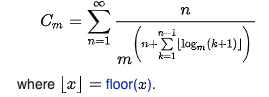
\includegraphics [scale=0.7]{images/formula.png} 

\section*{Characteristics and Applications} % Unnumbered section

The Champernowne’s constant has two important characteristics. First, any pattern of digits, no matter the content or length, will eventually appear in C10 [5].  An example of this is the number 456789 that occurs at position 2629624. In fact, the location of the pattern may be calculated [6][7]. Second, the nature of the Continued Fraction Expansion coefficients (CFE) of C10. The CFE consists mostly of coefficients with a reasonably small number of digits, interspersed with coefficients with a very large number of digits [8].

Some of the applications of the Champernowne’s constant include the use of its characteristics like the possibility to find every possible phrase (translated in binary string). For example, you can combine a normal number with some kind of instructions to find and extract that exactly matches the first Harry Potter novel (this is a copyright violation, but it is an interesting application). Additionally, it is also use by the comparison of the behavior of its digits with other numbers or elements. For example, if we compare a walk on the digits of Champernowne’s number with a walk on the nucleotides of a chromosome, such as the the X chromosome produces a similarly patterned image to the walk on the digits of Champernowne’s number [8].

%----------------------------------------------------------------------------------------
\begin{thebibliography}{9}

\bibitem{website} 
Champernowne Constant. (2019). Retrieved from: \\\texttt{http://oeis.org/search?q=Champernowne+constant\&sort=\&language=\&go=Search}

\bibitem{bib} 
D.G. Champernowne, The Construction of Decimals Normal in the Scale of Ten, J. London Math. Soc. 8, 1933, p. 254-260.
 
\bibitem{bib1} 
K. Mahler, Arithmetische Eigenschaften einer Klasse von Dezimalbrüchen, Proc. Konin. Neder. Akad. Wet. Ser. A. 40, 1937, p. 421-428.
 

\bibitem{website1} 
Transcendental Number. (2019). Retrieved from:  \\\texttt{http://mathworld.wolfram.com/TranscendentalNumber.html}

\bibitem{bib2} 
H. Von Baeyer, Information: The New Language of Science, Weidenfeld and Nicolson, Great Britain, 2003, p. 101-102, 104, 123-124. 

\bibitem{website2} 
Champernowne Constant. (2019). Retrieved from:  \\\texttt{http://www.infiniteabyss.org/2010/02/11/an\_interesting\_property\_of\_champernownes\_number.html}

\bibitem{website3} 
Champernowne Constant cfe Coefficient Calculation. (2019). Retrieved from: \\\texttt{http://code.google.com/p/champernowne-constant-cfe-coefficient-calculationhwm/downloads/list find\_num\_pos.rb}

\bibitem{website4} 
On the High Water Mark Convergents of Champernowne’s Constant in Base Ten. (2019). Retrieved from: \\\texttt{https://arxiv.org/pdf/1210.1263.pdf}

\bibitem{website5} 
AN INTERESTING PROPERTY OF CHAMPERNOWNE'S NUMBER.  (2019). Retrieved from: \\\texttt{https://www.kanonical.io/an\_interesting\_property\_of\_champernownes\_number/}
\end{thebibliography}

\end{document}
